\section{Descrição de Hardware}

O hardware do projeto foi projetado para realizar a medição contínua da temperatura e umidade do ambiente, garantindo que o microcontrolador seja capaz de alimentar o sensor e executar a lógica do sistema. A topologia eletrônica está dividida em cinco unidades principais, descritas a seguir.

\subsection*{Unidade de Controle}
A unidade de controle é a base do processamento lógico, sendo responsável por receber os dados, controlar os LEDs, o buzzer, o ventilador e o display, e se comunicar com a interface web. Foi selecionado o microcontrolador ESP32, que atende a esses requisitos graças à sua interface Wi-Fi 802.11 nativa e Bluetooth v4.2 BR/EDR. 

\begin{table}[h!]
    \centering
    \renewcommand{\arraystretch}{1.5}
    \begin{tabular}{|m{3.5cm}|m{3.5cm}|m{7cm}|}
        \hline
        \textbf{Componente} & \textbf{Imagem} & \textbf{Especificações Principais} \\
        \hline
        Microcontrolador ESP32 DevKit V1 & 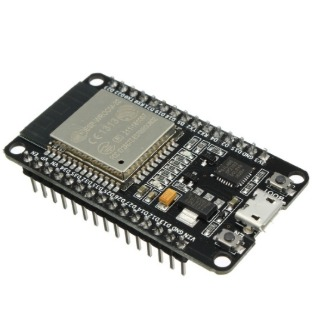
\includegraphics[width=2.5cm]{imag/esp32.png} & ROM: 448 KB. RAM: 520 KB. Conectividade: Wi-Fi 802.11 e Bluetooth v4.2 BR/EDR. \\
        \hline
    \end{tabular}
    \caption{Componente da unidade de controle.}
    \label{tab:unidade_controle}
\end{table}

\subsection*{Unidade de Aquisição de Dados}
Responsável por captar as condições ambientais, esta unidade utiliza o sensor DHT22, que envia temperatura e umidade ao ESP32 por um único fio digital. Para a exibição local dos dados, o projeto incorpora um display LCD 16x2 com módulo I\textsuperscript{2}C, que reduz a quantidade de pinos necessários para a comunicação com o microcontrolador.

\begin{table}[h!]
    \centering
    \renewcommand{\arraystretch}{1.5}
    \begin{tabular}{|m{3.5cm}|m{3.5cm}|m{7cm}|}
        \hline
        \textbf{Componente} & \textbf{Imagem} & \textbf{Especificações Principais} \\
        \hline
        Sensor DHT22 & 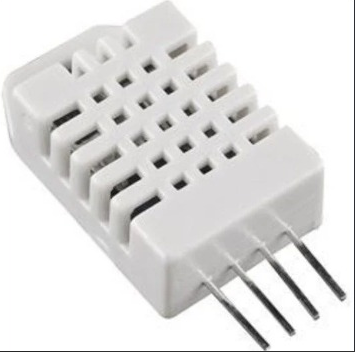
\includegraphics[width=2.5cm]{imag/sensor.PNG} & Tensão: 3,3 V a 5,5 V DC. Umidade: 0\% a 100\% RH. Saída digital de um fio. \\
        \hline
        Display LCD 16x2 (I\textsuperscript{2}C) & 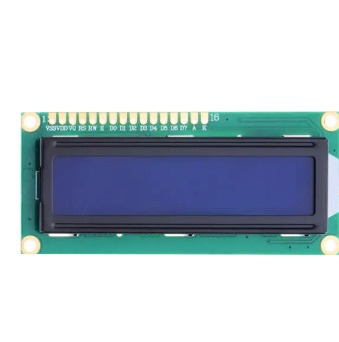
\includegraphics[width=2.5cm]{imag/display.png} & Tensão: 5 V DC. Comunicação: I\textsuperscript{2}C. Exibe temperatura, umidade e estado do sistema. \\
        \hline
    \end{tabular}
    \caption{Componentes da unidade de aquisição de dados.}
    \label{tab:unidade_aquisicao}
\end{table}

\subsection*{Unidade de Alimentação}
A energia do circuito é suprida por uma fonte de 5 V via conector USB, ligada diretamente ao ESP32. A própria placa já possui regulação de tensão, fornecendo os 3,3 V necessários ao microcontrolador e ao sensor, e por isso não é preciso um regulador externo. Para o ventilador, que necessita de 12 V, é feita uma derivação de alimentação separada.

\begin{table}[h!]
    \centering
    \renewcommand{\arraystretch}{1.5}
    \begin{tabular}{|m{3.5cm}|m{3.5cm}|m{7cm}|}
        \hline
        \textbf{Componente} & \textbf{Imagem} & \textbf{Especificações Principais} \\
        \hline
        Fonte USB 5 V & 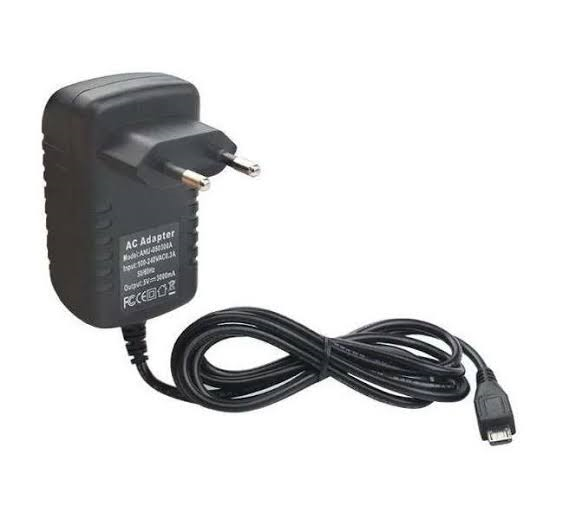
\includegraphics[width=2.5cm]{imag/fonte5v.png} & Tensão de entrada: 5 V via USB, que alimenta o ESP32 diretamente. \\
        \hline
    \end{tabular}
    \caption{Componente da unidade de alimentação.}
    \label{tab:unidade_alimentacao}
\end{table}

\subsection*{Bloco de Atuadores e Sinalização (Interfaces de Saída)}
Este bloco é responsável por informar o estado do sistema ao usuário e por atuar de forma autônoma na regulação do ambiente. Três LEDs (verde, amarelo e vermelho) fornecem a indicação visual, o buzzer emite o alerta sonoro e o ventilador promove a circulação forçada de ar.

\begin{table}[h!]
    \centering
    \renewcommand{\arraystretch}{1.5}
    \begin{tabular}{|m{3.5cm}|m{3.5cm}|m{7cm}|}
        \hline
        \textbf{Componente} & \textbf{Imagem} & \textbf{Especificações Principais} \\
        \hline
        LEDs de sinalização (verde, amarelo e vermelho) & \includegraphics[width=2.5cm]{imag/leds.png} & Queda de tensão direta: 1,8 V a 2,2 V (vermelho e amarelo) e 2,0 V a 2,2 V (verde). \\
        \hline
        Buzzer 5 V & 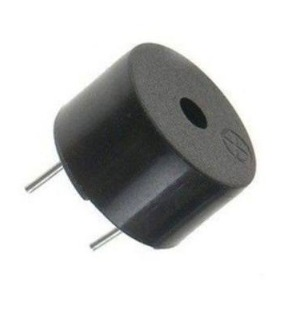
\includegraphics[width=2.5cm]{imag/buzzer.png} & Tensão: 4 V a 8 V. Corrente: $\sim$30 mA a 5 V. Alerta sonoro. \\
        \hline
        Ventilador DC 12 V & 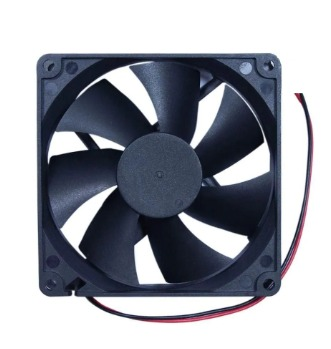
\includegraphics[width=2.5cm]{imag/ventilador.png} & Tensão: 12 V. Potência típica: $\sim$1,2 W a 2,4 W. \\
        \hline
    \end{tabular}
    \caption{Componentes do bloco de atuadores e sinalização.}
    \label{tab:atuadores}
\end{table}

\subsection*{Circuitos Auxiliares}
Os circuitos auxiliares garantem a correta polarização e a segurança do circuito principal. Resistores de 220\,$\Omega$ limitam a corrente dos LEDs e um resistor de 4,7\,k$\Omega$ funciona como \textit{pull-up} no barramento de dados do DHT22. O módulo relé isola o ESP32 do ventilador de 12\,V, protegendo o microcontrolador contra picos de tensão.

\begin{table}[h!]
    \centering
    \renewcommand{\arraystretch}{1.5}
    \begin{tabular}{|m{3.5cm}|m{3.5cm}|m{7cm}|}
        \hline
        \textbf{Componente} & \textbf{Imagem} & \textbf{Especificações Principais} \\
        \hline
        Resistores (220\,$\Omega$ e 4,7\,k$\Omega$) & 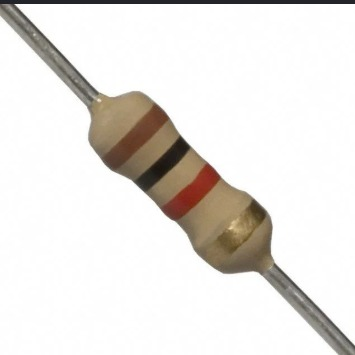
\includegraphics[width=2.5cm]{imag/resistor.png} & 220\,$\Omega$: limitação de corrente dos LEDs. 4,7\,k$\Omega$: \textit{pull-up} do sensor. \\
        \hline
        Módulo relé 5 V, 1 canal, com optoacoplador & 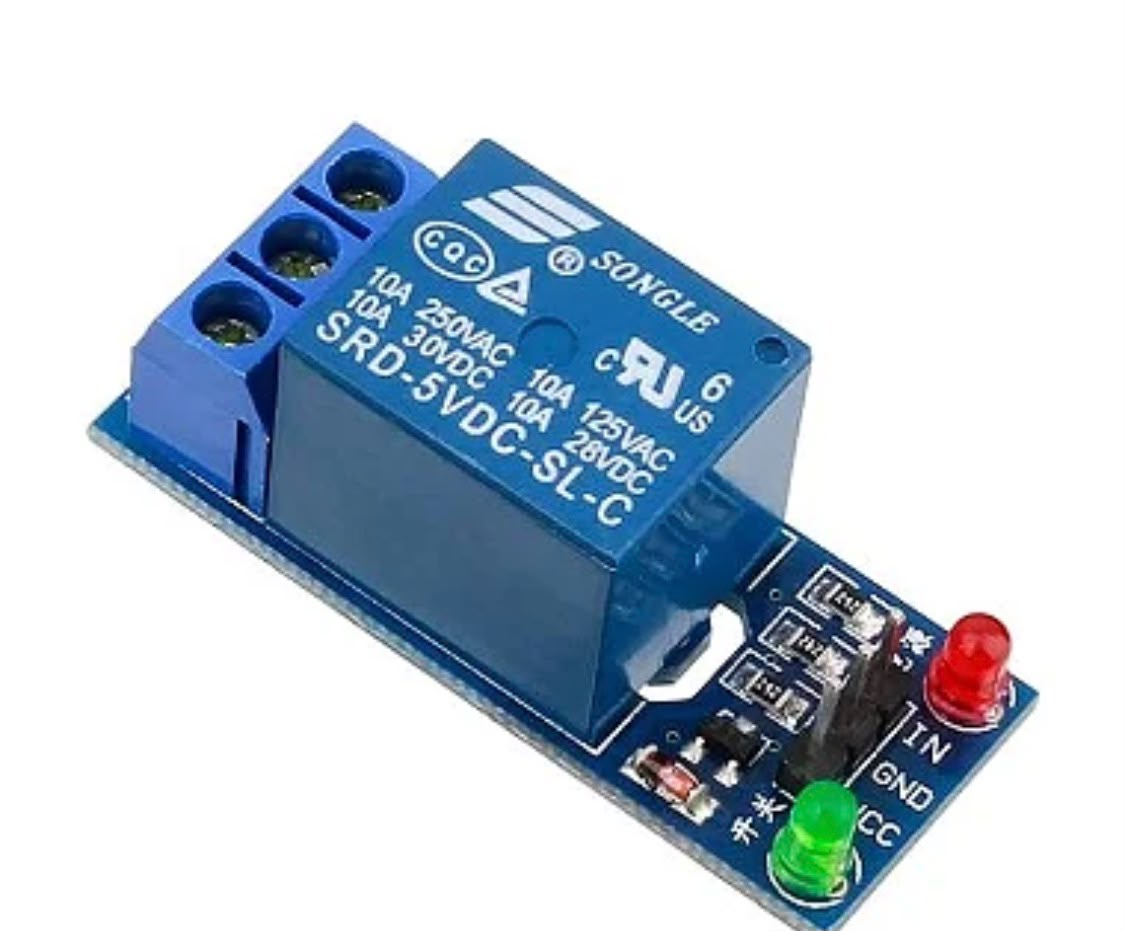
\includegraphics[width=2.5cm]{imag/rele.png} & Tensão de operação: 5 V DC. Sinal de controle: TTL 5 V. Capacidade: 30 V DC e 10 A ou 250 V AC e 10 A. Contatos NA e NF. \\
        \hline
    \end{tabular}
    \caption{Componentes dos circuitos auxiliares.}
    \label{tab:auxiliares}
\end{table}